\chapter{矩阵分解}\label{MathTools:chap:matrix_decomposition}
\section{LU分解}\label{MathTools:sec:lu_decomposition}
\section{QR分解及HouseHolder方法}\label{MathTools:sec:qr_decomposition}
\subsection{HouseHolder方法}\label{MathTools:sec:householder}
\section{SVD奇异值分解}\label{MathTools:sec:svd}
% todo : SVD奇异值分解搬运
\begin{theorembox}
	$A = U\Sigma V^T$,其中$U$和$V^T$是酉矩阵,$\Sigma$是对角线矩阵
\end{theorembox}
\subsubsection{SVD分解应用于PCA主成份分析}
https://www.cnblogs.com/daniel-D/p/3218063.html
\chapter{矩阵的逆及其求解方式}\label{MathTools:chap:matrix_inverse}
\section{LU分解求解对称正定矩阵的逆}\label{MathTools:sec:lu_inverse}
\section{QR分解求解右伪逆}\label{MathTools:sec:qr_pseudoinverse}
\section{SVD分解求广义逆}\label{MathTools:sec:svd_pseudoinverse}



\chapter{函数最优化问题求解方式}\label{MathTools:chap:optimization}
\section{原始牛顿法}\label{MathTools:sec:newton_method}
\section{雅可比矩阵和Hessian矩阵}\label{MathTools:sec:jacobian_hessian}
\section{高斯-牛顿法}\label{MathTools:sec:gauss_newton}
\section{拟牛顿法}\label{MathTools:sec:quasi_newton}
\subsection{Levenberg-Marquardt algorithm, LM}\label{MathTools:sec:lm}
\subsection{Davidon-Fletcher-Powell algoritm DFP}\label{MathTools:sec:dfp}
\subsection{Broyden–Fletcher–Goldfarb–Shanno algorithm BFGS}\label{MathTools:sec:bfgs}

\chapter{未分类}
\section{条件数}
条件数是线性方程组Ax=b的解对b中的误差或不确定度的敏感性的度量。数学定义为矩阵A的条件数等于A的范数与A的逆的范数的乘积,即cond(A)=‖A‖·‖A-1‖,对应矩阵的3种范数,相应地可以定义3种条件数。

matlab 里面运算函数:cond(A,2)或cond(A):2范数

一个极端的例子,当A奇异时,条件数为无穷,这时即使不改变b,x也可以改变。奇异的本质原因在于矩阵有0特征值,x在对应特征向量的方向上运动不改变Ax的值。如果一个特征值比其它特征值在数量级上小很多,x在对应特征向量方向上很大的移动才能产生b微小的变化,这就解释了为什么这个矩阵为什么会有大的条件数,事实上,正规阵在二范数下的条件数就可以表示成 abs(最大特征值/最小特征值)。——摘自百度百科

在计算机编程环境中,数据都是有浮点类型表示,精度有限,存在干扰,因此在解线性方程的时候都会存在误差。

\subsection{病态矩阵与条件数}
% todo : 条件数与病态矩阵
https://www.cnblogs.com/daniel-D/p/3219802.html
\subsubsection{与特征值和SVD的关系}
\subsubsection{病态矩阵的处理方法}
5. 病态矩阵处理方法
真正的自由是建立在规范的基础上的。病态矩阵解集的不稳定性是由于解集空间包含了自由度过大的方向,解决这个问题的关键就是将这些方向去掉,而保留 scaling 较大的方向,从而把解集局限在一个较小的区域内。在上面的讨论中, A 矩阵的特征向量不一定正交,不适合做新基, SVD 分解正好分解出了正交基,可以选前 k 个 $v^T$ 向量作为正交基。

比如,现在只选取前一个 (0.707, 0.707) 方向作为基,解集局限咋 y = x 这条直线上。直观的解释就是, A 矩阵的两个列向量过于类似,我们就可以将它们等同看待,第一次 b = (1000, 0), 解集是(0.5, 0.5), 第二次 b = (1000, 0.001), 解集还是 (0.5, 0.5).

总结起来,解决 A 病态就是将解集限定在一组正交基空间内,即对于坐标 y, 选择 k 个正交基 Zk,解决问题:$$\min_{y}\Vert AZ_ky - b \Vert ^2$$
这个就是 reduce-rank model. 具体方法有 truncated SVD 和 Krylov subspace method。
\section{带约束的最小范数解问题}
问题定义:
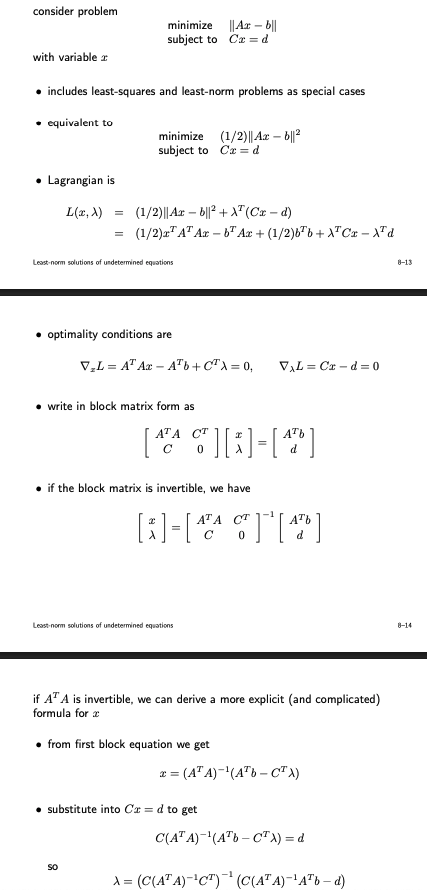
\includegraphics{MathTools/assets/rinv_with_constraints.png}
\begin{theorembox}
	$x = (A^TA)^{-1}(A^Tb-C^T(C(A^TA)^{-1}C^T)^{-1}(C(A^TA)^{-1}A^Tb-d))$
\end{theorembox}
\section{酉矩阵}
https://zh.wikipedia.org/wiki/%E9%85%89%E7%9F%A9%E9%98%B5
\subsection{图形中的稀疏表示}
% todo : 图形中的稀疏表示